The following are comparisions between wierdospace images produced in the
experiment, through the Monte Carlo simulation, and by analytic means.
Noise has been added to some of the analytic images to ``get you in the
right mood''.
\newpage
\begin{figure}
\begin{center}
\subfigure{
 \rput[r](-0.25,1.5){\parbox{2cm}{\begin{flushright}analytic\end{flushright}}}
 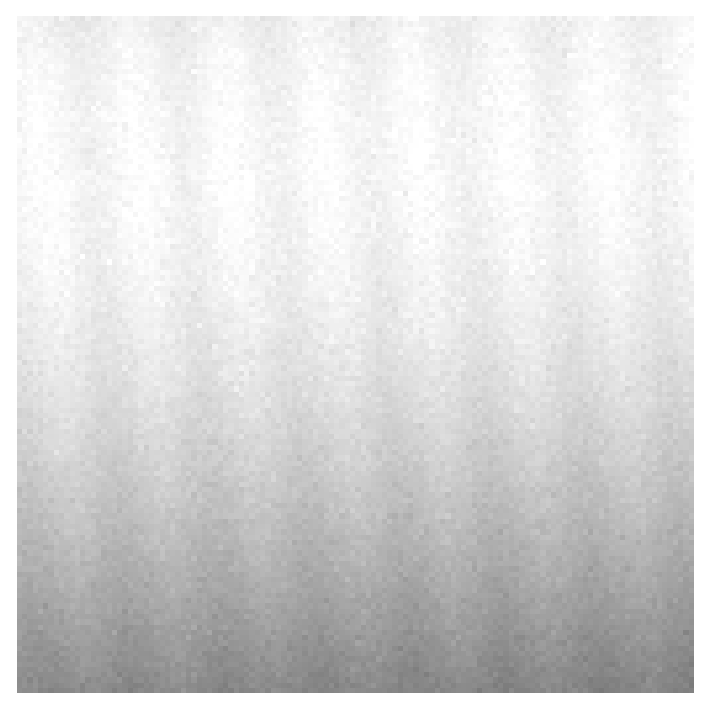
\includegraphics[width=3cm]{compare/allcmp/00180-theory.eps}}
\subfigure{
\includegraphics[width=3cm]{compare/allcmp/blank.eps}}
\subfigure{
\includegraphics[width=3cm]{compare/allcmp/blank.eps}}
\subfigure{
\includegraphics[width=3cm]{compare/allcmp/blank.eps}}\\
\subfigure{
 \rput[r](-0.25,1.5){\parbox{2cm}{\begin{flushright}Monte Carlo\end{flushright}}}
 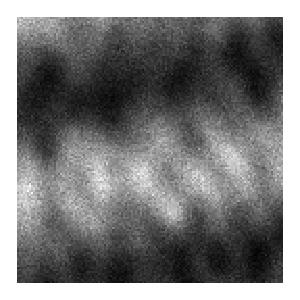
\includegraphics[width=3cm]{compare/allcmp/00180a-scatter.eps}}
\subfigure{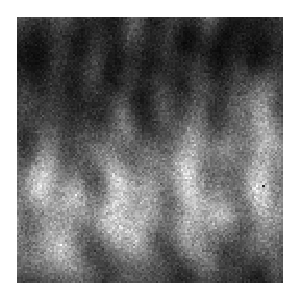
\includegraphics[width=3cm]{compare/allcmp/00180b-scatter.eps}}
\subfigure{
\includegraphics[width=3cm]{compare/allcmp/blank.eps}}
\subfigure{
\includegraphics[width=3cm]{compare/allcmp/blank.eps}}\\
\setcounter{subfigure}{0}
\subfigure{
 \rput[r](-0.25,1.5){\parbox{2cm}{\begin{flushright}experiment\end{flushright}}}
 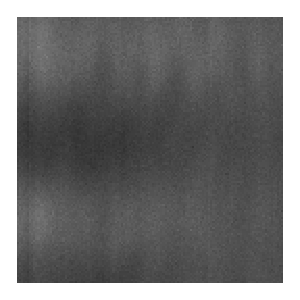
\includegraphics[width=3cm]{compare/allcmp/00180-01368_circ414.eps}}
\subfigure{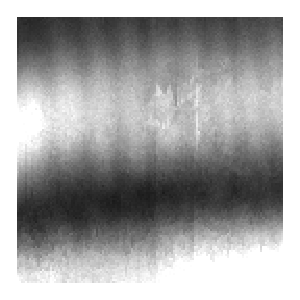
\includegraphics[width=3cm]{compare/allcmp/00180-01441_circ434.eps}}
\subfigure{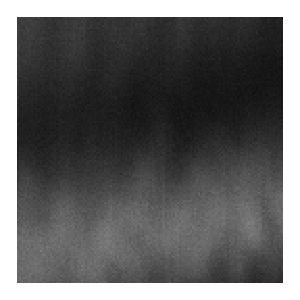
\includegraphics[width=3cm]{compare/allcmp/00180-01495_circ646.eps}}
\subfigure{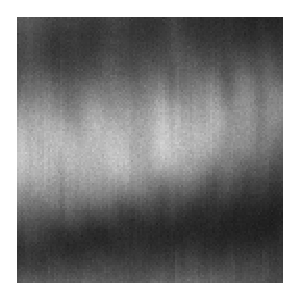
\includegraphics[width=3cm]{compare/allcmp/00180-01576_circ559.eps}}
\end{center}
\caption{Comparison of analytic, Monte Carlo, and experimental weirdospace
in the vicinity of the \SI{180}{\degree} scattering direction.  The
vertical features are secondary stripes produced by Equation \ref{eqn:cbs}.}
\label{fig:scat180degree}
\end{figure}

\begin{figure}
\centering
\subfigure[Monte Carlo]{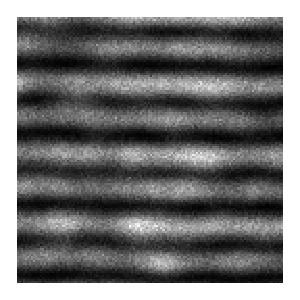
\includegraphics[width=3cm]{compare/allcmp/00002-scatter.eps}}
\subfigure[analytic]{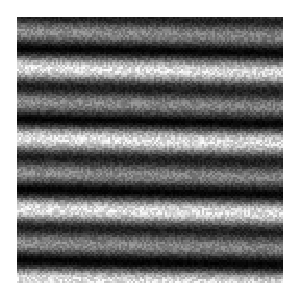
\includegraphics[width=3cm]{compare/allcmp/00002-theory.eps}}
\caption{Comparison of Monte Carlo and analytic weirdospace in the
vicinity of the \SI{0}{\degree} scattering direction.  The alternating
intensity pattern is an interference between primary stripes and the two
Type \Rmnum{3} events.}
\label{fig:scat0degree}
\end{figure}

\begin{figure}
\centering
\subfigure{
 \rput[r](-0.25,1.5){\parbox{2cm}{\begin{flushright}analytic\end{flushright}}}
 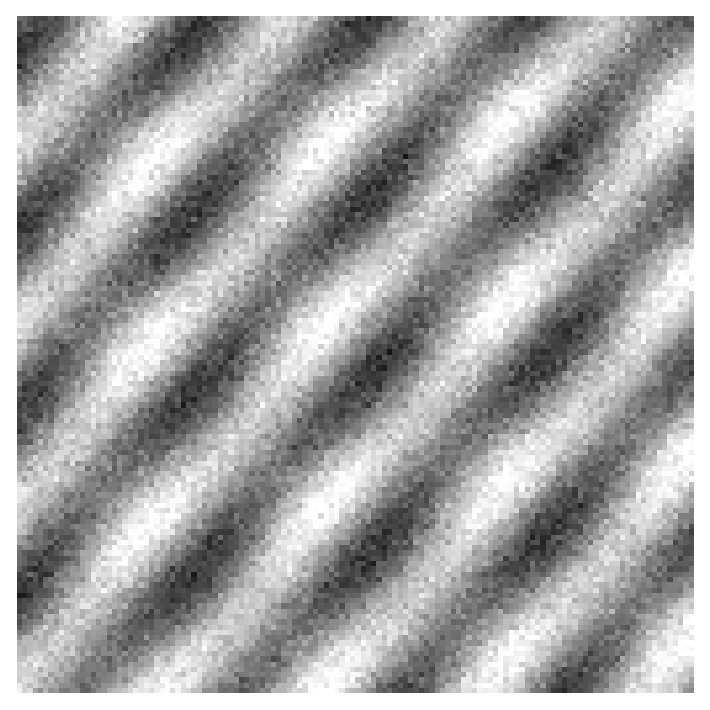
\includegraphics[width=3cm]{compare/allcmp/00085-theory.eps}}
\subfigure{
\includegraphics[width=3cm]{compare/allcmp/blank.eps}}\\
\subfigure{
 \rput[r](-0.25,1.5){\parbox{2cm}{\begin{flushright}Monte Carlo\end{flushright}}}
 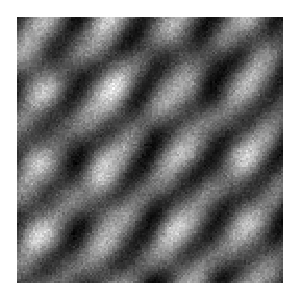
\includegraphics[width=3cm]{compare/allcmp/00085-scatter.eps}}
\subfigure{
\includegraphics[width=3cm]{compare/allcmp/blank.eps}}\\
\subfigure{
 \rput[r](-0.25,1.5){\parbox{2cm}{\begin{flushright}experiment\end{flushright}}}
 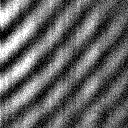
\includegraphics[width=3cm]{compare/allcmp/00085-00982_circ427}}
\subfigure{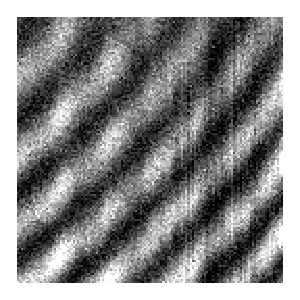
\includegraphics[width=3cm]{compare/allcmp/00085-01100_circ647}}
\caption{Comparison of analytic, Monte Carlo, and experimental weirdospace
in the vicinity of the \SI{85}{\degree} scattering direction.  Note the
distinct shape of the dark pockets predicted by the analytic and Monte
Carlo simulations.  This shape is due to interference of the two Type
\Rmnum{3} events.}
\label{fig:scat85degree}
\end{figure}

\begin{figure}
\centering
\subfigure{
 \rput[r](-0.25,1.5){\parbox{2cm}{\begin{flushright}analytic\end{flushright}}}
 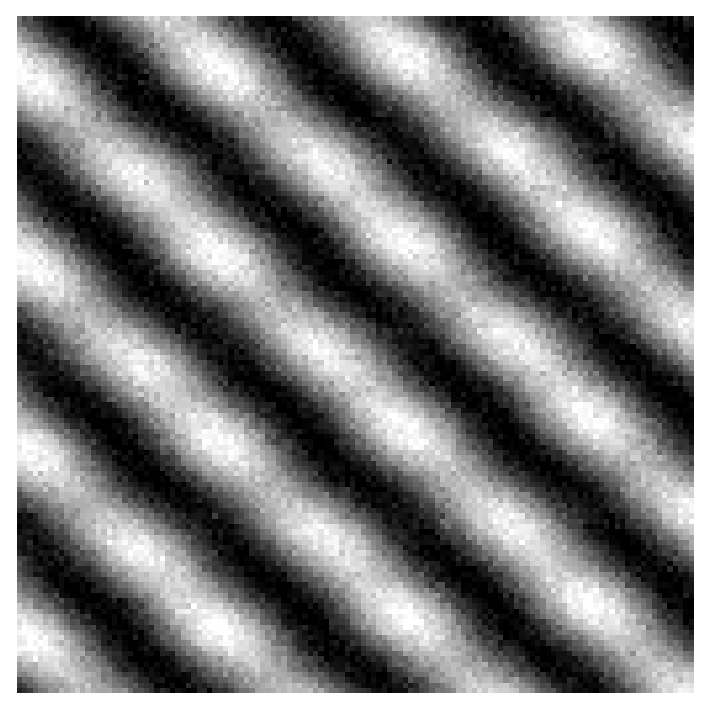
\includegraphics[width=3cm]{compare/allcmp/00270-theory.eps}}
\subfigure{
\includegraphics[width=3cm]{compare/allcmp/blank.eps}}\\
\subfigure{
 \rput[r](-0.25,1.5){\parbox{2cm}{\begin{flushright}Monte Carlo\end{flushright}}}
 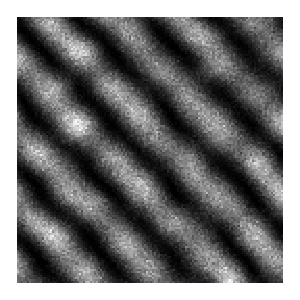
\includegraphics[width=3cm]{compare/allcmp/00270-scatter.eps}}
\subfigure{
\includegraphics[width=3cm]{compare/allcmp/blank.eps}}\\
\subfigure{
 \rput[r](-0.25,1.5){\parbox{2cm}{\begin{flushright}experiment\end{flushright}}}
 
\includegraphics[width=3cm]{compare/allcmp/00270-00111_circ647.eps}}
\subfigure{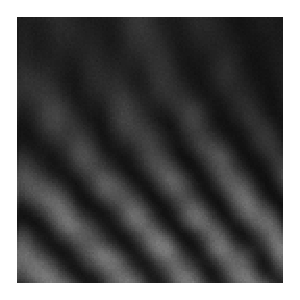
\includegraphics[width=3cm]{compare/allcmp/00270-00188_circ515.eps}}
\caption{Comparison of analytic, Monte Carlo, and experimental weirdospace
in the vicinity of the \SI{270}{\degree} scattering direction.  Note the
orientation of the secondary stripes and that they come in intensity groups
of two.}
\label{fig:scat270degree}
\end{figure}

\begin{figure}
\begin{center}
\addtolength{\subfigbottomskip}{-1cm}
 \psset{unit=1cm}
\subfigure{
 \rput[r](-0.25,1.5){\parbox{2cm}{\begin{flushright}analytic, $E_\chi$ not included\end{flushright}}}
 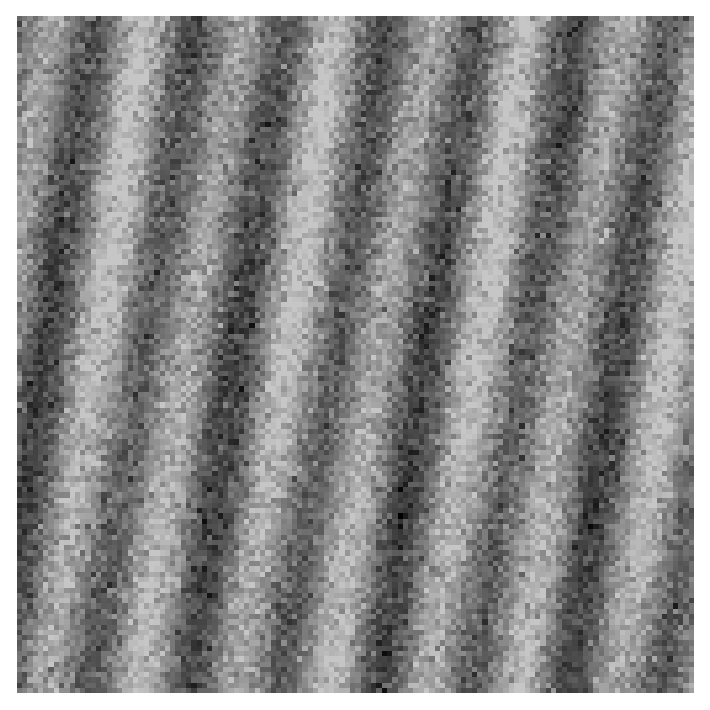
\includegraphics[width=3cm]{compare/allcmp/cbs-00016-theory.eps}}
\subfigure{ 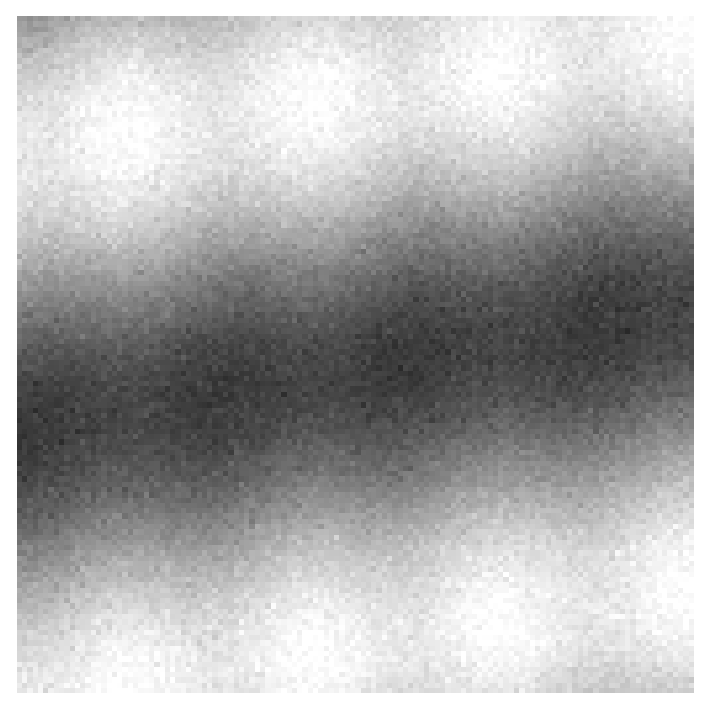
\includegraphics[width=3cm]{compare/allcmp/cbs-00160-theorya.eps}}
\subfigure{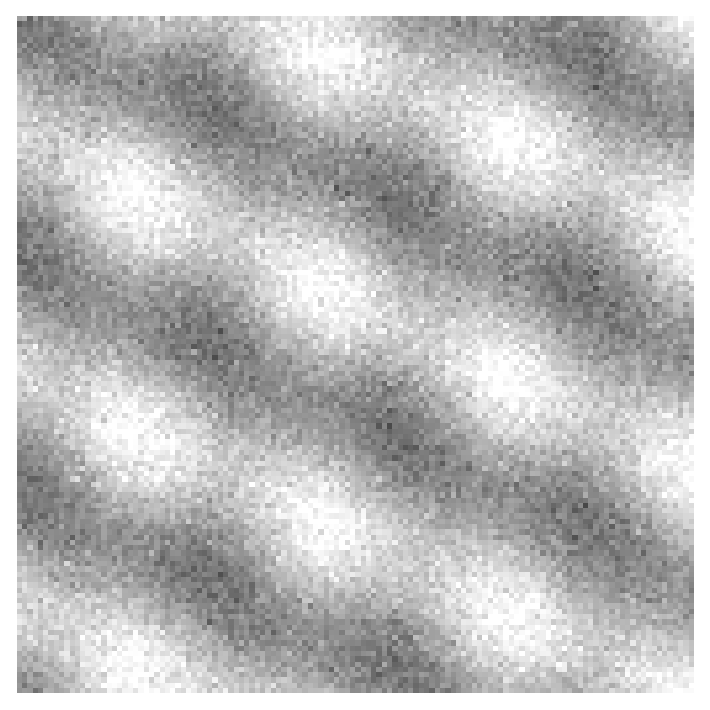
\includegraphics[width=3cm]{compare/allcmp/cbs-00233-theorya.eps}}\\
\subfigure{
 \rput[r](-0.25,1.5){\parbox{2cm}{\begin{flushright}Monte Carlo, no time reverse paths.\end{flushright}}}
 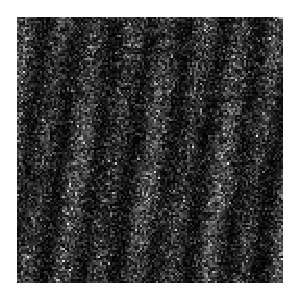
\includegraphics[width=3cm]{compare/allcmp/cbs-00016-scatter-notr.eps}}
\subfigure{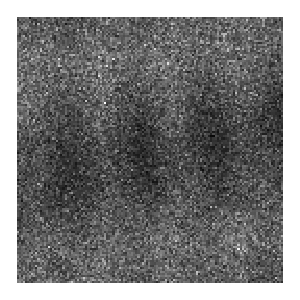
\includegraphics[width=3cm]{compare/allcmp/cbs-00160-scatter-notr.eps}}
\subfigure{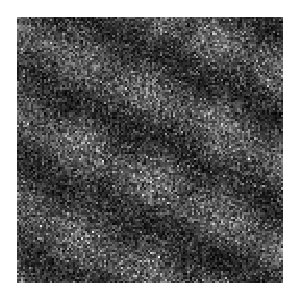
\includegraphics[width=3cm]{compare/allcmp/cbs-00233-scatter-notr.eps}}\\
\subfigure{
 \rput[r](-0.25,1.5){\parbox{2cm}{\begin{flushright}analytic, $E_\chi$ included\end{flushright}}}
 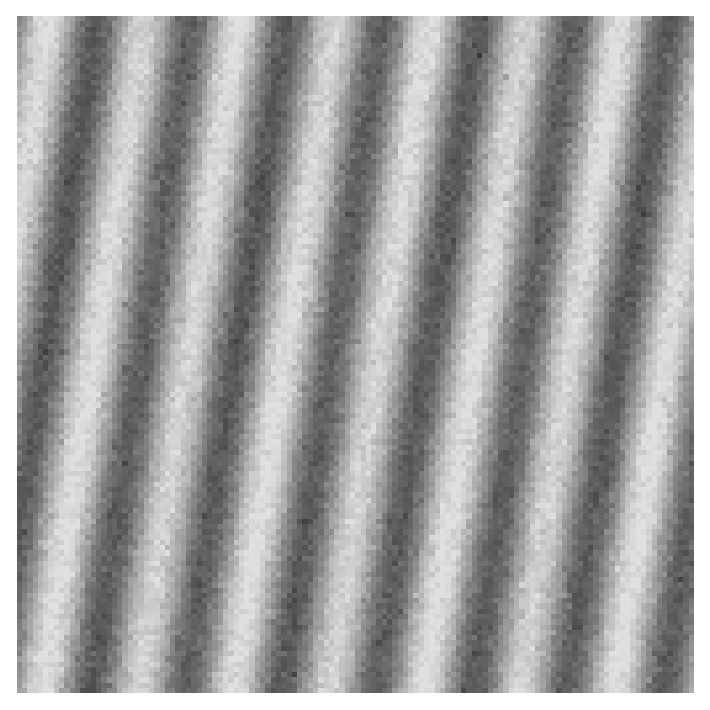
\includegraphics[width=3cm]{compare/allcmp/cbs-00016-theoryb.eps}}
\subfigure{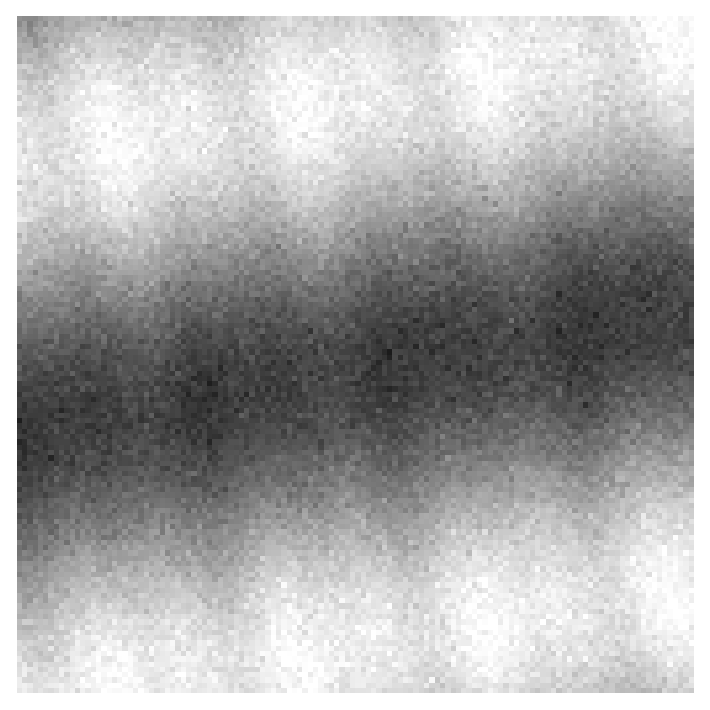
\includegraphics[width=3cm]{compare/allcmp/cbs-00160-theoryb.eps}}
\subfigure{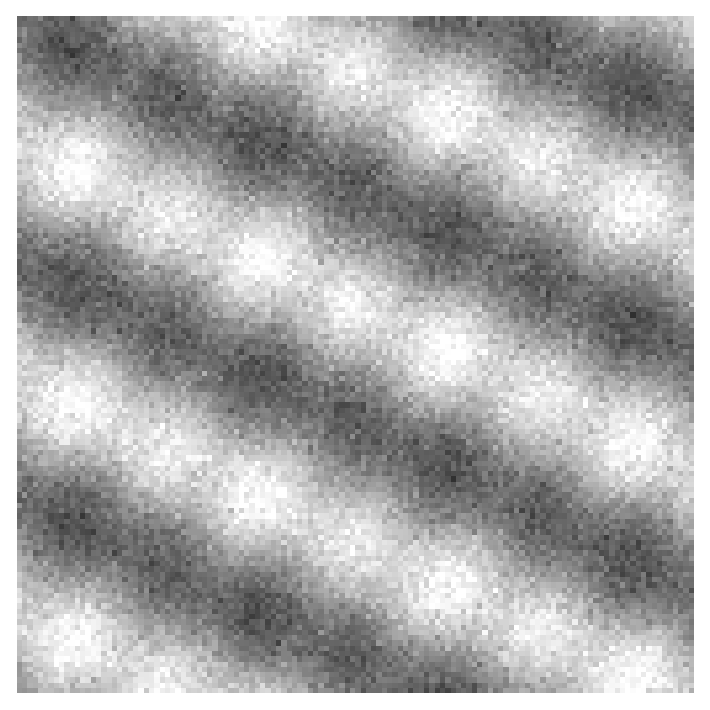
\includegraphics[width=3cm]{compare/allcmp/cbs-00233-theoryb.eps}}\\
\setcounter{subfigure}{0}
\subfigure[\SI{16}{\degree}]{
 \rput[r](-0.25,1.5){\parbox{2cm}{\begin{flushright}Monte Carlo, time reverse paths included.\end{flushright}}}
 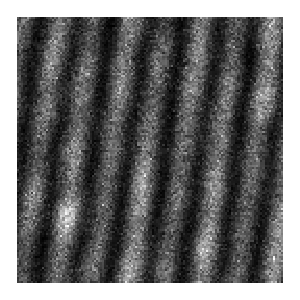
\includegraphics[width=3cm]{compare/allcmp/cbs-00016-scatter-withtr.eps}}
\subfigure[\SI{160}{\degree}]{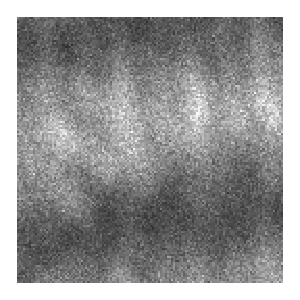
\includegraphics[width=3cm]{compare/allcmp/cbs-00160-scatter-withtr.eps}}
\subfigure[\SI{233}{\degree}]{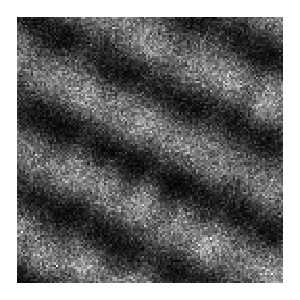
\includegraphics[width=3cm]{compare/allcmp/cbs-00233-scatter-withtr.eps}}\\
\end{center}
\caption{Comparison of analytic and Monte Carlo simulations in the case
where time reverse paths (Equation \ref{eqn:cbs}) have been removed from
either.}
\label{fig:rtr}
\end{figure}

\begin{figure}
\centering
\subfigure[analytic]{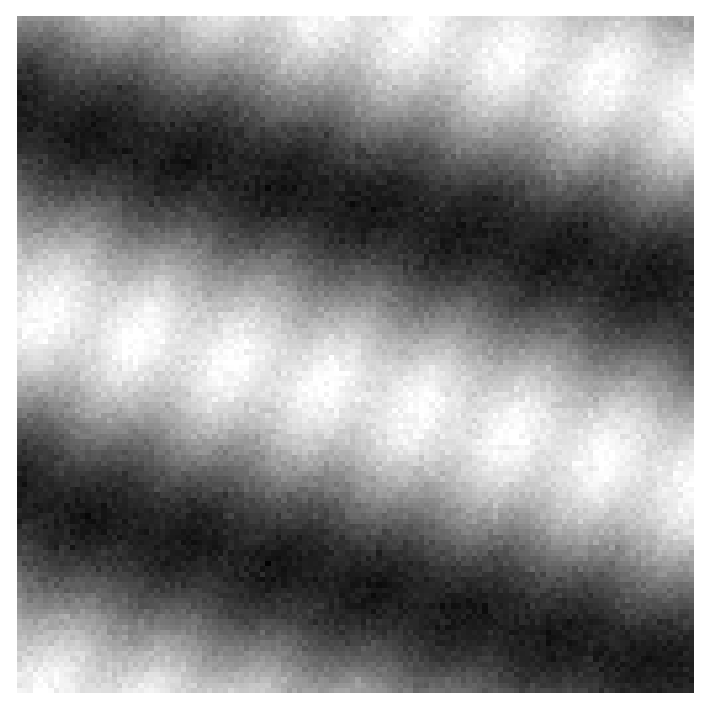
\includegraphics[width=3cm]{compare/allcmp/d1-theory.eps}}
\subfigure[Monte Carlo]{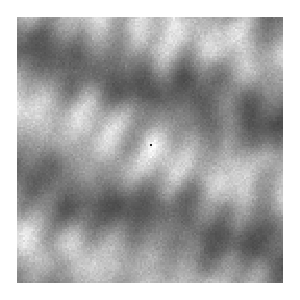
\includegraphics[width=3cm]{compare/allcmp/d1-00213-scatter.eps}}
\subfigure[experiment]{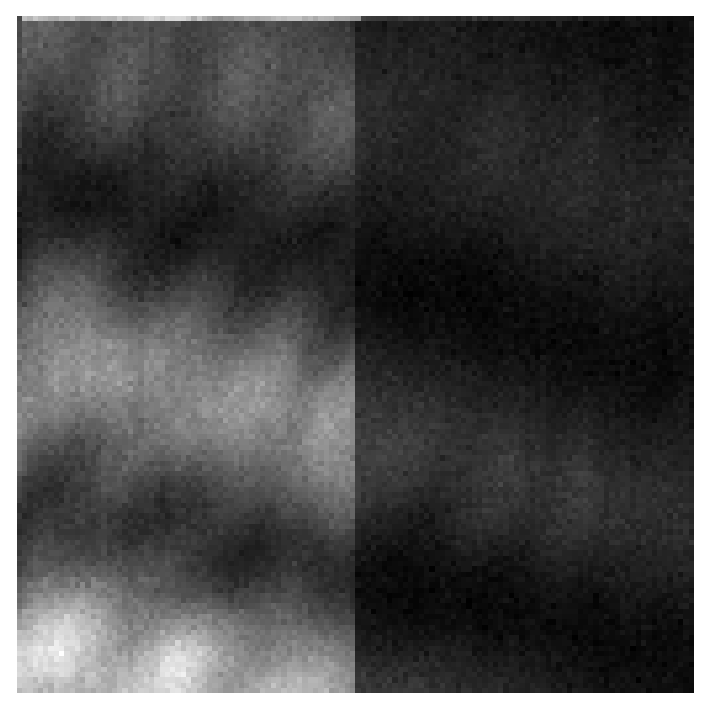
\includegraphics[width=3cm]{compare/allcmp/d1-experiment.eps}}
\caption{Comparison of analytic and experimental weirdospace for some angle
around the ring.  Note the relationship between intensity maxima on each
primary stripe and their ``hexagonal packing'' relationship.  Also, the way
these maxima connects with another with a thin, curvy intensity.  This
interference effect is from primary and secondary stripes.}
\label{fig:hexagonalpacking1}
\end{figure}

\begin{figure}
\centering
\subfigure[scan538]{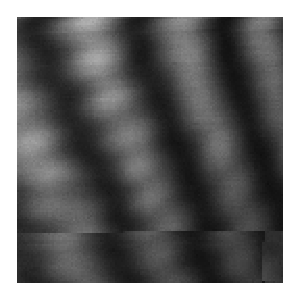
\includegraphics[width=3cm]{compare/allcmp/o1-00000_circ538.eps}}
\subfigure[scan645]{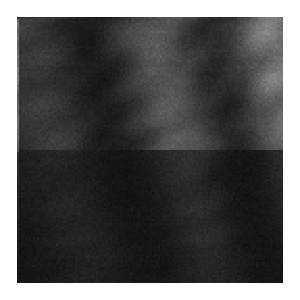
\includegraphics[width=3cm]{compare/allcmp/o1-01795_circ645.eps}}
\subfigure[scan645]{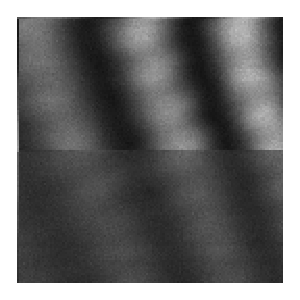
\includegraphics[width=3cm]{compare/allcmp/o1-01843_circ645.eps}}
\caption{Exhibition of some of the stripe features found in the
experimental data.  Note the (alternating) relationship between intensity
maxima on each primary stripe and their ``hexagonal packing''. This
interference effect is from primary and secondary stripes.}
\label{fig:hexagonalpacking2}
\end{figure}
